\documentclass{beamer}

\usepackage{graphicx}
\usepackage{hyperref}
\usepackage{xcolor}
\usepackage{listings}
\usepackage{textcomp}
\usepackage{svg}
\graphicspath{pics/}
% Theme choice
\usetheme{Madrid}

% Title Page
\title{Pro.wiz AI Project Plan}
\author{Nithin Vadekkapat}
\institute{DhvaniAI}
\date{\today}

\begin{document}

% Title Slide
\begin{frame}
    \titlepage
\end{frame}

\section{Overview}
\begin{frame}
    \sectionpage
\end{frame}

% Slide: Background
\begin{frame}{Background}
    \begin{itemize}
        \item We are building an AI-powered Project Management \& ERP solution designed for Design \& Engineering businesses.
        \item The solution, Pro.wiz, will leverage AI from the beginning to solve common issues in project execution.
        \item It will be a cloud-based service, billed based on the data volume processed.
    \end{itemize}
\end{frame}

% Slide: Target Audience
\begin{frame}{Target Audience}
    \begin{itemize}
        \item Design \& Engineering businesses in sectors such as:
        \begin{itemize}
            \item Oil \& Gas
            \item Infrastructure Development
            \item Chemical \& Process Industries
            \item Power Generation
            \item Water \& Effluent Treatment
            \item Aviation, Food \& Beverage, Marine \& Shipbuilding
        \end{itemize}
        \item Ideal fit: Businesses with annual billing between \$50M and \$150M.
        \item These companies handle multiple projects, generate and revise numerous documents, and require compliance and safety verification.
    \end{itemize}
\end{frame}

% Slide: AI Integration \& Requirements
\begin{frame}{AI Integration \& Requirements}
    \begin{itemize}
        \item Our in-house team will build the ERP system, but we require AI expertise to accelerate implementation.
        \item A specialized team is needed to:
        \begin{itemize}
            \item Evaluate AI models and select the most appropriate one.
            \item Train an SLM model on business-specific data.
            \item Automate time-consuming engineering tasks.
            \item Ensure seamless integration via API endpoints using JSON.
        \end{itemize}
        \item Data sources include historical contracts, drawings, standards, QC procedures, and business process documentation.
    \end{itemize}
\end{frame}
\section{Usecases}
\begin{frame}
    \sectionpage
\end{frame}
% Slide: Input and Output Documents Table
\begin{frame}{Usecase 1: Preparation of Equipment List \& Datasheets}
    \begin{table}[h]
        \begin{tabular}{|l|l|}
        \hline
        \textbf{Input Documents} & \textbf{Output Documents} \\ 
        \hline
        P\&IDs & Equipment List \\ 
        Mechanical Design Basis& Manual Control Valve List \\ 
        Project specifications &  Mechanical Datasheets \\ 
        Piping Material Specifications &  \\ 
        Valve Material Specifications &  \\ 
        Painting Specifications &  \\ 
        Insulation Specifications &  \\
        Pressure Vessel Specifications &  \\
        Material Specifications &  \\ 
        \hline
        \end{tabular}
        \caption{Input and Output Documents for f Equipment List \& Datasheets}
    \end{table}
\end{frame}

% Slide: Instrument Index and I/O List Documents
\begin{frame}{Usecase 2: Input and Output Documents for Instrument Index and I/O List}
    \begin{table}[]
        \centering
        \begin{tabular}{|l|l|}
            \hline
            \textbf{Input Documents} & \textbf{Output Documents} \\
            \hline
            Piping and Instrumentation Diagrams (P\&IDs) & Instrument I/O List \\
            Alarm Trip Schedule & Instrument Index \\
            Line List & \\
            \hline
        \end{tabular}
        \caption{Input and Output Documents for Instrument Index and I/O List}
    \end{table}
\end{frame}

% Slide: Preparation of Instrument Datasheets
\begin{frame}{Usecase 3: Preparation of Instrument Datasheets}
    \begin{itemize}
        \item Instrument datasheets are prepared by extracting data from:
        \begin{itemize}
            \item Instrument Index
            \item Piping and Instrumentation Diagrams (P\&IDs)
            \item Instrument Specifications
        \end{itemize}
        \item This data is fed into standard templates.
    \end{itemize}
\end{frame}

% Slide: Structural and Civil Cost Estimation
\begin{frame}{Usecase 4: Structural and Civil Cost Estimation}
    \begin{itemize}
        \item Automatic generation of BOQs and cost estimation.
        \item Covers RCC buildings and steel sheds.
        \item Based on cost database and standard estimation formats.
    \end{itemize}
\end{frame}
% Slide: Codes & Standards Referencing
\begin{frame}{Usecase 5: Codes \& Standards Referencing}
    \begin{itemize}
        \item Retrieve relevant clauses from standards (ASTM, ASME, API, ISO, etc.).
        \item Summarize and explain sections from standards.
        \item Provide cross-references between different standards.
        \item Automated compliance checks of engineering documents.
    \end{itemize}
\end{frame}

\section{DhvaniAI Solution}
\begin{frame}
    \sectionpage
\end{frame}

\begin{frame}{Usecase Architecture}
        \centering
        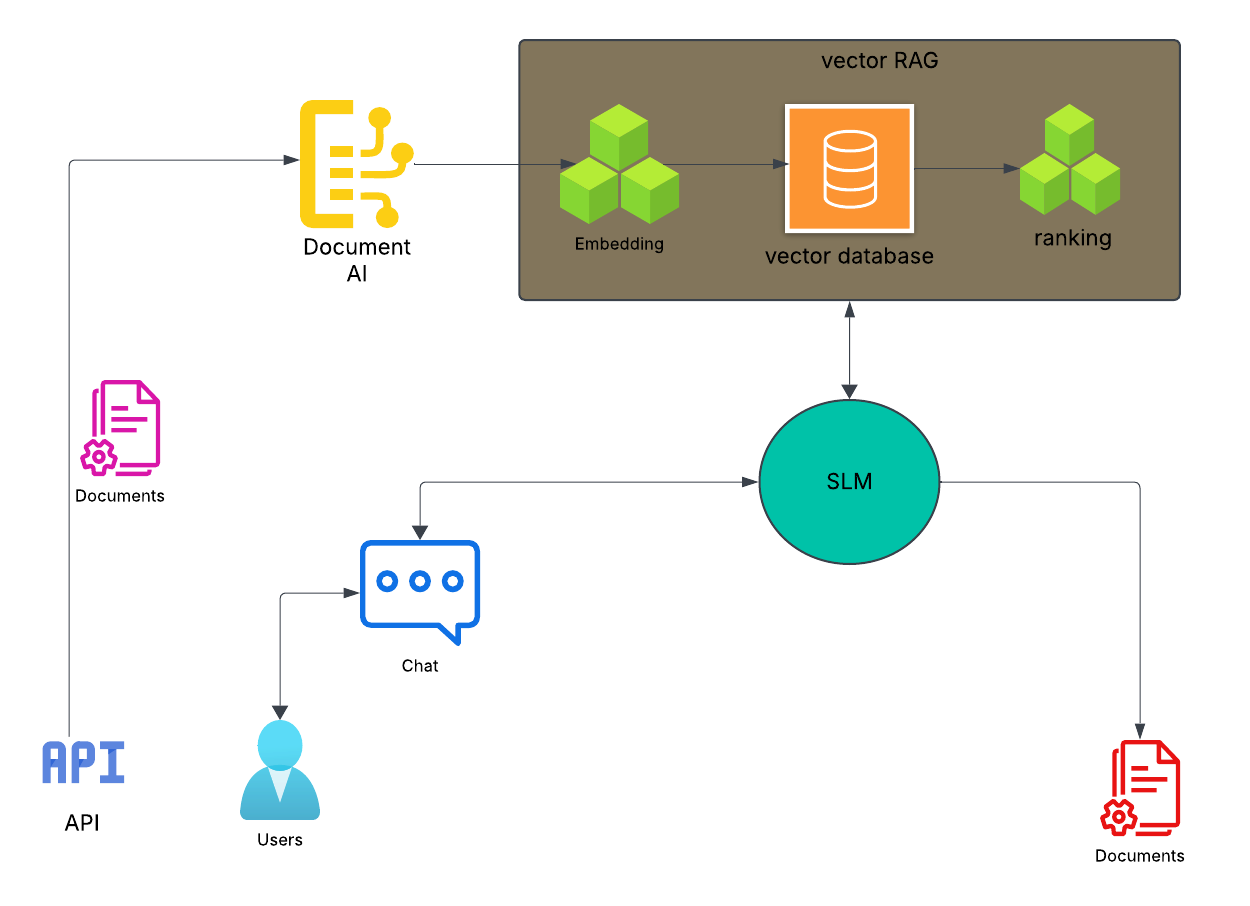
\includegraphics[width=0.9\textwidth]{pics/diagram.png}
\end{frame}

\begin{frame}{Agentic Architecture}
    \centering
    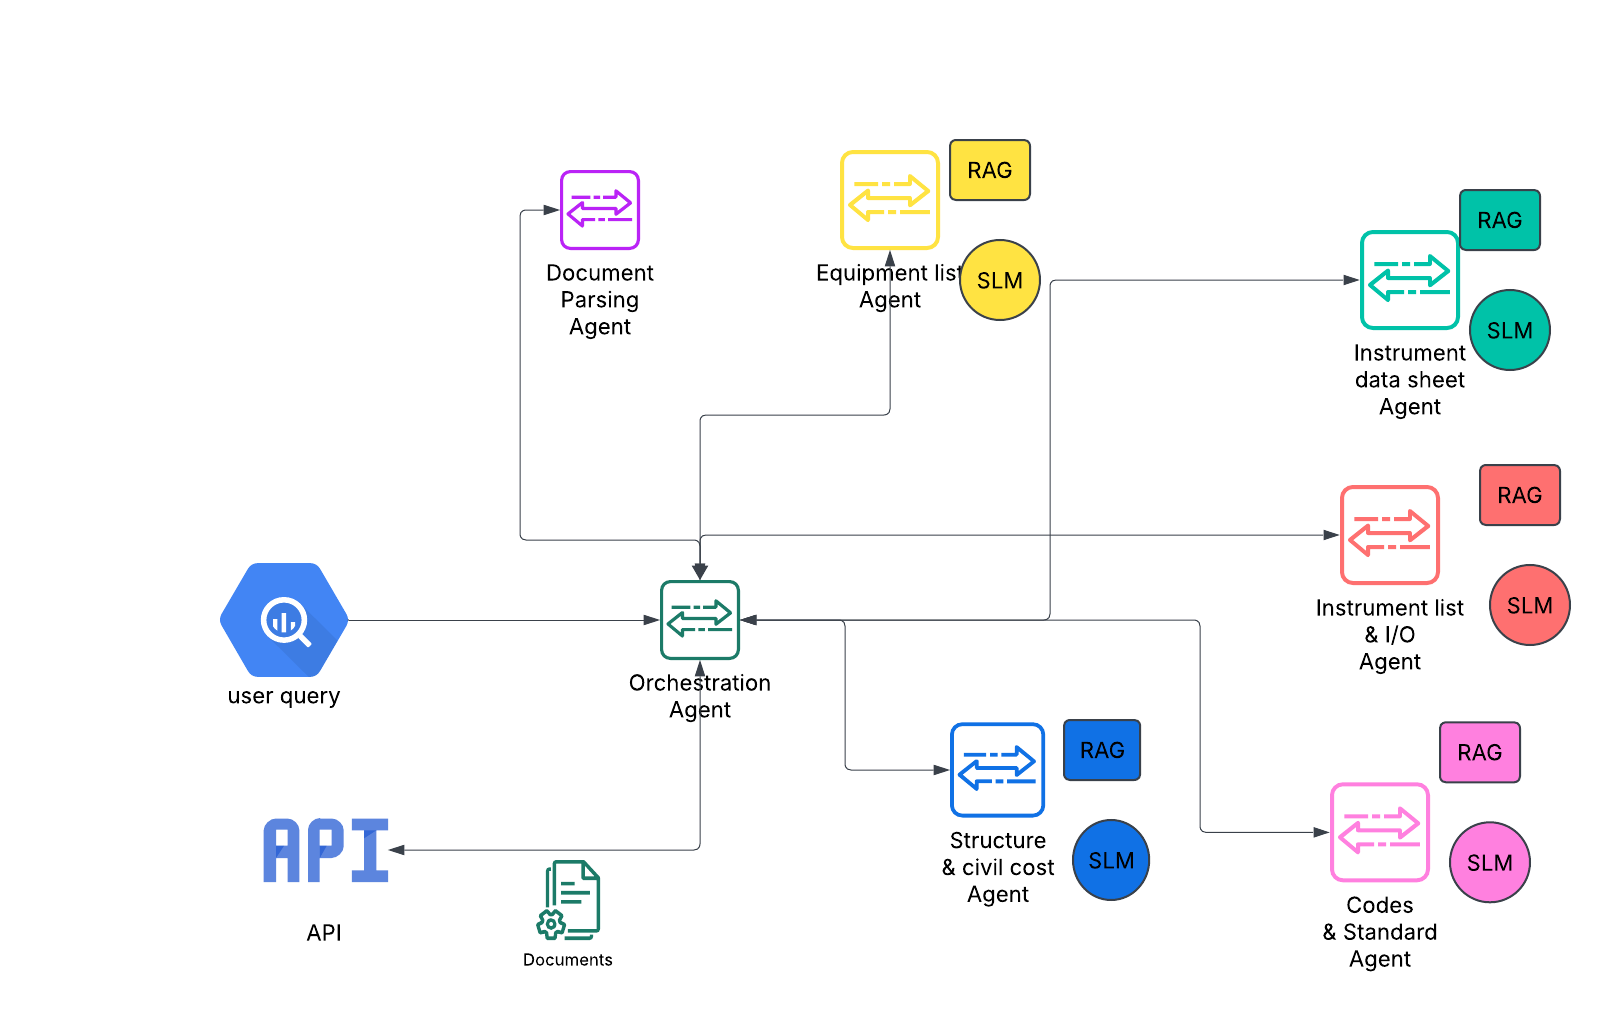
\includegraphics[width=0.9\textwidth]{pics/agentic.png}
\end{frame}


\section{Project Plan}                                                                    
\end{document}



